\documentclass[landscape,paperwidth=40in,paperheight=30in,margin=1in]{baposter}

\usepackage{calc}
\usepackage{graphicx}
\usepackage{amsmath}
\usepackage{amssymb}
\usepackage{relsize}
\usepackage{multirow}
\usepackage{rotating}
\usepackage{bm}
\usepackage{url}

\usepackage{graphicx}
\usepackage{multicol}

%\usepackage{times}
%\usepackage{helvet}
%\usepackage{bookman}
\usepackage{palatino}

\newcommand{\captionfont}{\footnotesize}

\graphicspath{{images/}{../images/}}
\usetikzlibrary{calc}

% my imports
\usetikzlibrary{bayesnet}
\usepackage{booktabs}
\usepackage{makecell}

% my commands
\newcommand{\argmax}[1]{\underset{#1}{\text{arg max }}}
\newcommand{\Bin}[1]{\text{Binomial}(#1)}
\newcommand{\Bern}[1]{\text{Bernoulli}(#1)}
\newcommand{\Bet}[1]{\text{Beta}(#1)}
\newcommand{\Cat}[1]{\text{Categorical}(#1)}
\newcommand{\const}{\text{ const }}
\newcommand{\Dir}[1]{\text{Dirichlet}(#1)}
\newcommand{\E}[1]{\underset{#1}{\mathbb{E}}}
\newcommand{\iid}{\overset{iid}{\sim}}
\newcommand{\ictr}{\mathbf{1}}
\newcommand{\maximum}[1]{\underset{#1}{\text{max }}}
\newcommand{\Uni}[1]{\text{Uniform}(#1)}

\newcommand{\SET}[1]  {\ensuremath{\mathcal{#1}}}
\newcommand{\MAT}[1]  {\ensuremath{\boldsymbol{#1}}}
\newcommand{\VEC}[1]  {\ensuremath{\boldsymbol{#1}}}
\newcommand{\Video}{\SET{V}}
\newcommand{\video}{\VEC{f}}
\newcommand{\track}{x}
\newcommand{\Track}{\SET T}
\newcommand{\LMs}{\SET L}
\newcommand{\lm}{l}
\newcommand{\PosE}{\SET P}
\newcommand{\posE}{\VEC p}
\newcommand{\negE}{\VEC n}
\newcommand{\NegE}{\SET N}
\newcommand{\Occluded}{\SET O}
\newcommand{\occluded}{o}

%%%%%%%%%%%%%%%%%%%%%%%%%%%%%%%%%%%%%%%%%%%%%%%%%%%%%%%%%%%%%%%%%%%%%%%%%%%%%%%%
%%%% Some math symbols used in the text
%%%%%%%%%%%%%%%%%%%%%%%%%%%%%%%%%%%%%%%%%%%%%%%%%%%%%%%%%%%%%%%%%%%%%%%%%%%%%%%%

%%%%%%%%%%%%%%%%%%%%%%%%%%%%%%%%%%%%%%%%%%%%%%%%%%%%%%%%%%%%%%%%%%%%%%%%%%%%%%%%
% Multicol Settings
%%%%%%%%%%%%%%%%%%%%%%%%%%%%%%%%%%%%%%%%%%%%%%%%%%%%%%%%%%%%%%%%%%%%%%%%%%%%%%%%
\setlength{\columnsep}{1.5em}
\setlength{\columnseprule}{0mm}

%%%%%%%%%%%%%%%%%%%%%%%%%%%%%%%%%%%%%%%%%%%%%%%%%%%%%%%%%%%%%%%%%%%%%%%%%%%%%%%%
% Save space in lists. Use this after the opening of the list
%%%%%%%%%%%%%%%%%%%%%%%%%%%%%%%%%%%%%%%%%%%%%%%%%%%%%%%%%%%%%%%%%%%%%%%%%%%%%%%%
\newcommand{\compresslist}{%
\setlength{\itemsep}{1pt}%
\setlength{\parskip}{0pt}%
\setlength{\parsep}{0pt}%
}

%%%%%%%%%%%%%%%%%%%%%%%%%%%%%%%%%%%%%%%%%%%%%%%%%%%%%%%%%%%%%%%%%%%%%%%%%%%%%%
%%% Begin of Document
%%%%%%%%%%%%%%%%%%%%%%%%%%%%%%%%%%%%%%%%%%%%%%%%%%%%%%%%%%%%%%%%%%%%%%%%%%%%%%

\begin{document}

%%%%%%%%%%%%%%%%%%%%%%%%%%%%%%%%%%%%%%%%%%%%%%%%%%%%%%%%%%%%%%%%%%%%%%%%%%%%%%
%%% Here starts the poster
%%%---------------------------------------------------------------------------
%%% Format it to your taste with the options
%%%%%%%%%%%%%%%%%%%%%%%%%%%%%%%%%%%%%%%%%%%%%%%%%%%%%%%%%%%%%%%%%%%%%%%%%%%%%%
% Define some colors

%\definecolor{lightblue}{cmyk}{0.83,0.24,0,0.12}
\definecolor{lightblue}{rgb}{0.145,0.6666,1}

\hyphenation{resolution occlusions}
%%
\begin{poster}%
  % Poster Options
  {
  % Show grid to help with alignment
  grid=false,
  % Column spacing
  colspacing=1em,
  % Color style
  bgColorOne=white,
  bgColorTwo=white,
  borderColor=lightblue,
  headerColorOne=black,
  headerColorTwo=lightblue,
  headerFontColor=white,
  boxColorOne=white,
  boxColorTwo=lightblue,
  % Format of textbox
  textborder=roundedleft,
  % Format of text header
  eyecatcher=true,
  headerborder=closed,
  headerheight=0.1\textheight,
%  textfont=\sc, An example of changing the text font
  headershape=roundedright,
  headershade=shadelr,
  headerfont=\large\bf\textsc, %Sans Serif
  textfont={\setlength{\parindent}{1.5em}},
  boxshade=plain,
%  background=shade-tb,
  background=plain,
  linewidth=2pt
  }
  % Eye Catcher
  {
    \begin{tabular}{cc}
         
\includegraphics[height=8.0em]{images/columbia_university.png}
         &
         
\includegraphics[height=8.0em]{images/cs_cu.png}
    \end{tabular}
    } 
  % Title
  {\bf\textsc{Neural Inverse CDF Sampling}\vspace{0.5em}}
  % Authors
  {\textsc{Andrew Stirn: }andrew.stirn@columbia.edu\\
   \textsc{Tony Jebara: }jebara@cs.columbia.edu}
  % University logo
  {% The makebox allows the title to flow into the logo, this is a hack because of the L shaped logo.
    
\includegraphics[height=8.0em]{images/Netflix_Logo_RGB.png}
  }

%%%%%%%%%%%%%%%%%%%%%%%%%%%%%%%%%%%%%%%%%%%%%%%%%%%%%%%%%%%%%%%%%%%%%%%%%%%%%%
%%% Now define the boxes that make up the poster
%%%---------------------------------------------------------------------------
%%% Each box has a name and can be placed absolutely or relatively.
%%% The only inconvenience is that you can only specify a relative position 
%%% towards an already declared box. So if you have a box attached to the 
%%% bottom, one to the top and a third one which should be in between, you 
%%% have to specify the top and bottom boxes before you specify the middle 
%%% box.
%%%%%%%%%%%%%%%%%%%%%%%%%%%%%%%%%%%%%%%%%%%%%%%%%%%%%%%%%%%%%%%%%%%%%%%%%%%%%%
    %
    % A coloured circle useful as a bullet with an adjustably strong filling
    \newcommand{\colouredcircle}{%
      \tikz{\useasboundingbox (-0.2em,-0.32em) rectangle(0.2em,0.32em); \draw[draw=black,fill=lightblue,line width=0.03em] (0,0) circle(0.18em);}}

%%%%%%%%%%%%%%%%%%%%%%%%%%%%%%%%%%%%%%%%%%%%%%%%%%%%%%%%%%%%%%%%%%%%%%%%%%%%%%
  \headerbox{The Problem}{name=problem,column=0,row=0}{
%%%%%%%%%%%%%%%%%%%%%%%%%%%%%%%%%%%%%%%%%%%%%%%%%%%%%%%%%%%%%%%%%%%%%%%%%%%%%%
	Variational Bayesian inference frequently relies on Monte Carlo (MC) integration when intractable expectations appear in the evidence lower bound (ELBO). Variational inference evaluates these expectations wrt the proposed posterior approximations. In many cases, such as in Variational Auto-Encoders, we maximize the ELBO via gradient methods, however, to do so in conjunction MC integration requires that samples from the posterior approximations are differentiable wrt their respective parameters. Closed-form ``reparameterization tricks'' unfortunately only exist for a subset of distribution families (e.g. Gaussian).
 }

%%%%%%%%%%%%%%%%%%%%%%%%%%%%%%%%%%%%%%%%%%%%%%%%%%%%%%%%%%%%%%%%%%%%%%%%%%%%%%
  \headerbox{Inverse CDF Sampling}{name=inv_cdf,column=0,row=0,below=problem}{
%%%%%%%%%%%%%%%%%%%%%%%%%%%%%%%%%%%%%%%%%%%%%%%%%%%%%%%%%%%%%%%%%%%%%%%%%%%%%%
    For continuous univariate distribution, inverse CDF sampling allows us to reparameterize a sample from a Uniform distribution to the target distribution:
	\begin{equation*}
	\begin{aligned}
		\epsilon &\sim \Uni{0,1}\\
		z &= F^{-1}(\epsilon; \ \theta) 
	\end{aligned}
	\end{equation*}	 
	Unfortunately, not all continuous univariate distributions have a closed form quantile function, $F^{-1}$. In these cases, $\frac{\partial z}{\partial \theta}$ does not exist, prohibiting gradient methods.
  }
%%%%%%%%%%%%%%%%%%%%%%%%%%%%%%%%%%%%%%%%%%%%%%%%%%%%%%%%%%%%%%%%%%%%%%%%%%%%%%
  \headerbox{Our Contributions}{name=contributions,column=0,row=0,below=inv_cdf}{
%%%%%%%%%%%%%%%%%%%%%%%%%%%%%%%%%%%%%%%%%%%%%%%%%%%%%%%%%%%%%%%%%%%%%%%%%%%%%%
    We leverage invertible neural network (INN) blocks \cite{ref:inn} to approximate continuous univariate CDF's, allowing for inverse CDF sampling while ensuring the existence of $\frac{\partial z}{\partial \theta}$. Because the INN blocks are analytically invertible, our approximation maintains \emph{monotonicity} and \emph{one-to-oneness} thus ensuring: $z = F^{-1}(F(z;\theta);\theta)$. 
  }
%%%%%%%%%%%%%%%%%%%%%%%%%%%%%%%%%%%%%%%%%%%%%%%%%%%%%%%%%%%%%%%%%%%%%%%%%%%%%%
  \headerbox{Invertible Neural Network}{name=inn,column=1, span=2}{
%%%%%%%%%%%%%%%%%%%%%%%%%%%%%%%%%%%%%%%%%%%%%%%%%%%%%%%%%%%%%%%%%%%%%%%%%%%%%%
	Affine coupling layer \cite{ref:inn}
	\begin{center}	
	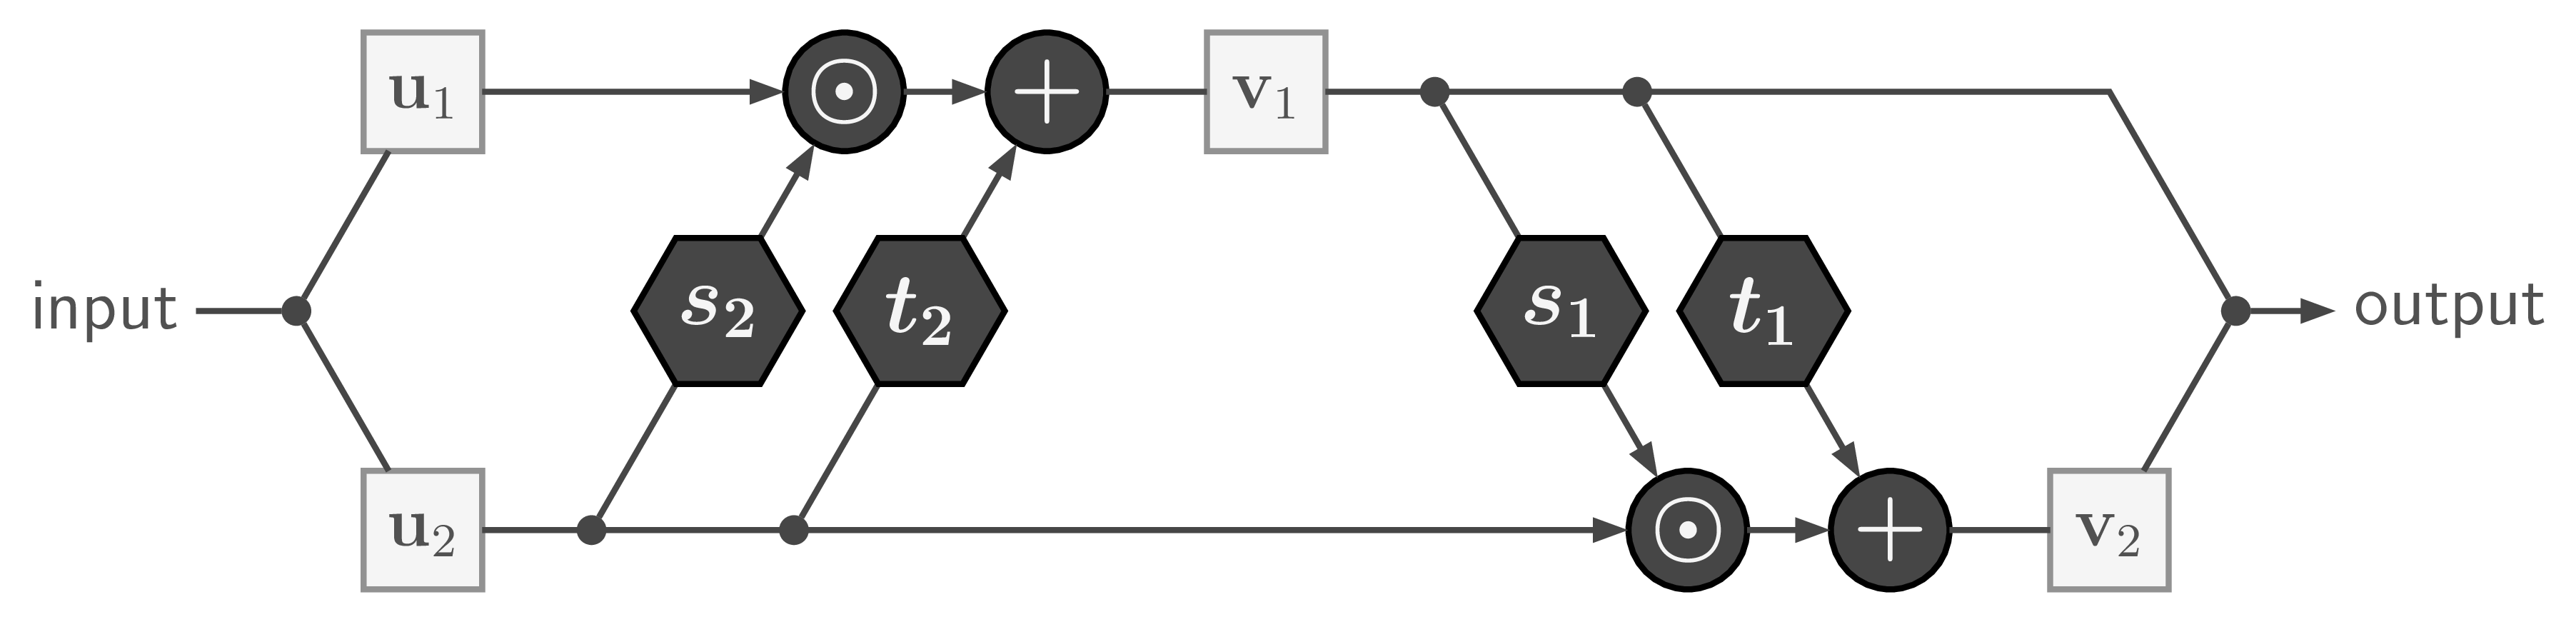
\includegraphics[width=\columnwidth]{images/inn_forward.png}
	\\
	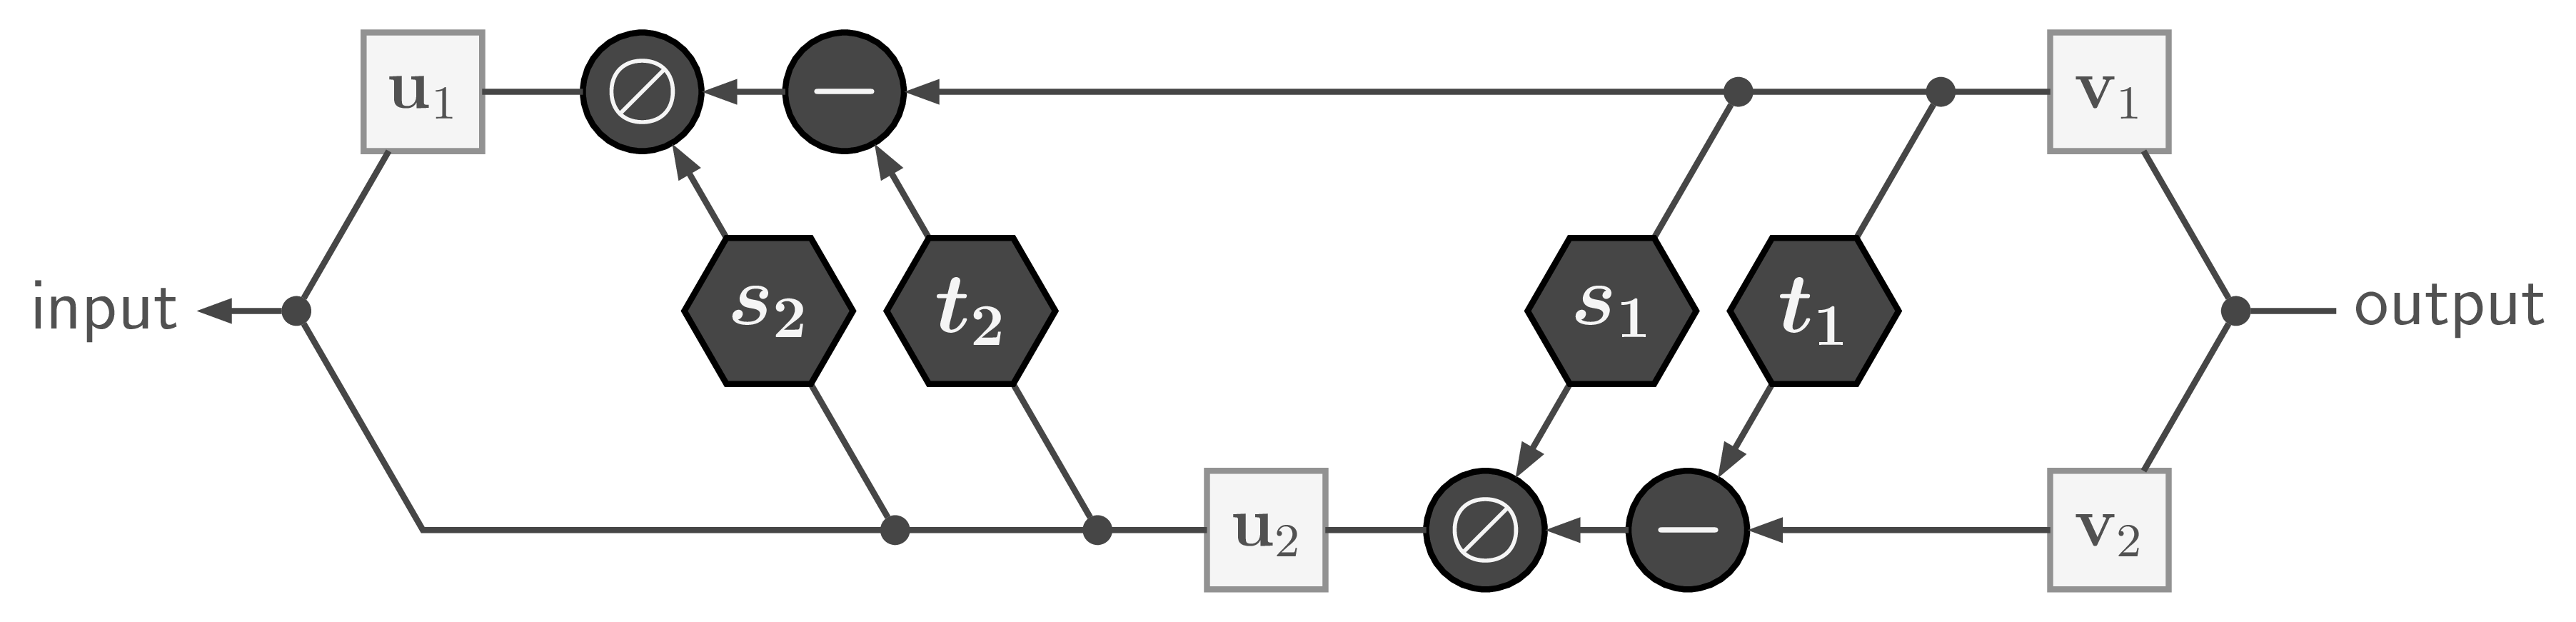
\includegraphics[width=\columnwidth]{images/inn_backward.png}
	\end{center}
  }
  
%%%%%%%%%%%%%%%%%%%%%%%%%%%%%%%%%%%%%%%%%%%%%%%%%%%%%%%%%%%%%%%%%%%%%%%%%%%%%%
  \headerbox{CDF Approximation for Gamma Distribution}{name=gamma_results,column=1, span=2, below=inn}{
%%%%%%%%%%%%%%%%%%%%%%%%%%%%%%%%%%%%%%%%%%%%%%%%%%%%%%%%%%%%%%%%%%%%%%%%%%%%%%
	\centering
	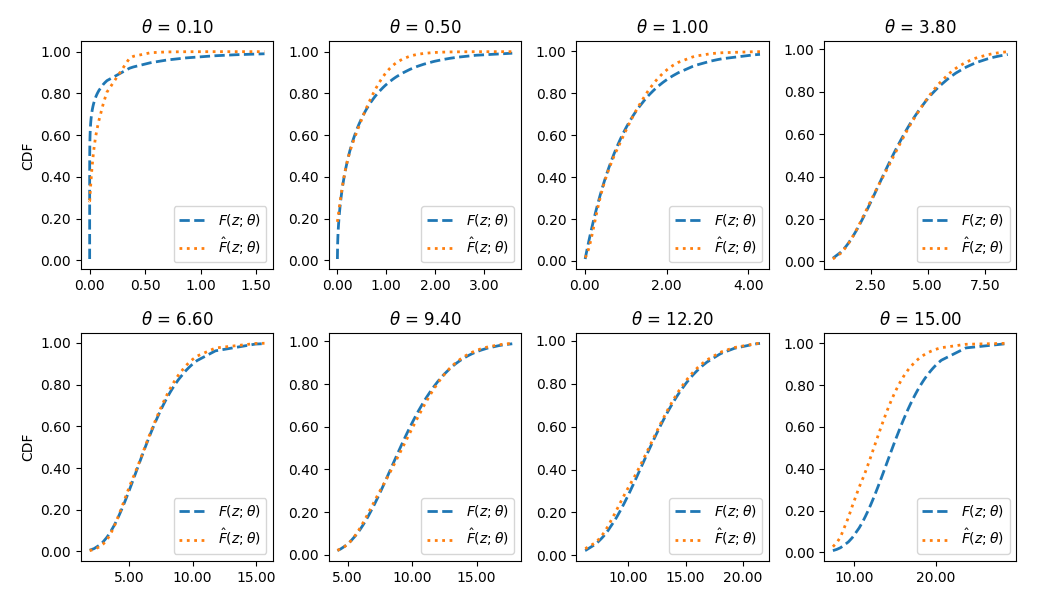
\includegraphics[width=\columnwidth]{images/nicdf_Gamma.png}
}

%%%%%%%%%%%%%%%%%%%%%%%%%%%%%%%%%%%%%%%%%%%%%%%%%%%%%%%%%%%%%%%%%%%%%%%%%%%%%%
\headerbox{Gradient Reparameterization}{name=algorithms,column=3,row=0}{
%%%%%%%%%%%%%%%%%%%%%%%%%%%%%%%%%%%%%%%%%%%%%%%%%%%%%%%%%%%%%%%%%%%%%%%%%%%%%%
	\centering
	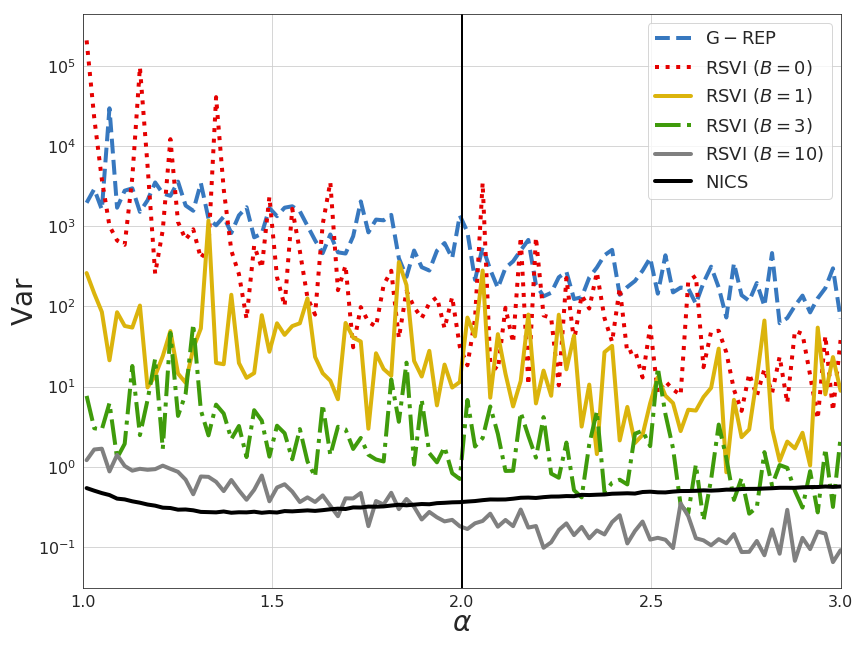
\includegraphics[width=\columnwidth]{images/gradientVariance.png}
}

%%%%%%%%%%%%%%%%%%%%%%%%%%%%%%%%%%%%%%%%%%%%%%%%%%%%%%%%%%%%%%%%%%%%%%%%%%%%%%
\headerbox{Results}{name=lda,column=3,below=algorithms}{
%%%%%%%%%%%%%%%%%%%%%%%%%%%%%%%%%%%%%%%%%%%%%%%%%%%%%%%%%%%%%%%%%%%%%%%%%%%%%%
  \begin{tabular}{ccc}
    \multicolumn{3}{c}{Perplexity Scores}\\
    \toprule
    				& Softmax		& NGS\\
    \midrule
    NVLDA		& 1099.96		& 1103.77\\
    \midrule
    ProDLDA		& 1161.69		& 1099.94\\
    \midrule
  \end{tabular}
  }

%%%%%%%%%%%%%%%%%%%%%%%%%%%%%%%%%%%%%%%%%%%%%%%%%%%%%%%%%%%%%%%%%%%%%%%%%%%%%%
  \headerbox{References \& Code}{name=references,column=3,span=1,below=lda}{
%%%%%%%%%%%%%%%%%%%%%%%%%%%%%%%%%%%%%%%%%%%%%%%%%%%%%%%%%%%%%%%%%%%%%%%%%%%%%%
    \smaller
    \renewcommand{\section}[2]{\vskip 0.05em}
    \bibliographystyle{plain}
    {\tiny \bibliography{references}}
    Source code available at:\\
    \url{github.com/astirn/neural-inverse-cdf-sampling}
  }
  

\end{poster}

\end{document}
